%matplotlib inline: esto es para que las graficas aparescan a dentro.

\documentclass{article}
%Reporte de computacional
%matplotlib inline: esto es para que las graficas aparescan a dentro.
\usepackage{hyperref}
\usepackage{amsmath}
\usepackage{amsthm}
\usepackage{amssymb}
\usepackage{graphicx}
\usepackage{ifxetex}
\ifxetex
\usepackage{fontspec}
\else
\usepackage[T1]{fontenc}
\usepackage[utf8]{inputec}
\usepackage{lmodern}
\fi



\begin{document}
\title{Sistemas de masas con oscilaciones no lineales y forzadas}
\author{Ramses Pacheco Ortiz}
\date{14 De abril Del 2018}
\maketitle  


\section{Introducción}

Esta practica es continuacion de la actividad 6 que incluyen las seciones 1 y 2 del articulo llamado "coupled springs equations" de los autores Fay y Graham,en donde se vio un sistema de resortes acoplado.

En esta actividad abordaremos el resto de las secciones de este articulo, especificamente la seccion 3 y 4, en donde cada seccion tiene su nivel de complejidad por ejemplo,en la seccion 3 toman consideraciones y fuerzas no lineales, esto quiere decir que no es proporcional al  desplazamiento y por lo tanto trabajaremos ecuaciones no linenales.

Por otro lado en la seccion 4 es similar a la seccion 3 pero tomando otras consideraciones como un forzamiento externos dando soluciones de $cos wt$ llamdas soluciones harmonicas o en tal caso subharmonicas.

\section{añadiendo no-linealidad}

En esta parte del articulo realizamos varia suposiciones,por ejemplño, Si suponemos que las fuerzas de restauración no son lineales, lo que sin duda es cierto para grandes vibraciones,donde la fuerza de restauración es de la forma $F=-kx$ (ley de Hooke), la cual no describe correctamente el sistema acopaldo,por que lo podemos considerar que la fuerza de restauración tiene la forma $f=kx+ux3$. Entonces de nuestro modelo se deducen las siguientes ecuaciones:

\begin{center}
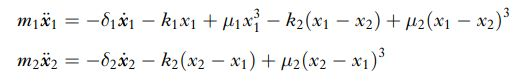
\includegraphics[height=3cm]{ec14.png}
\end{center}

%%%%%%%%%%%%%%%%%%%%%%%%%%%%%%%%%%%%%%%%%%%%%%%

\subsection{Ejemplo 3.1}

Suponga que $m1=m2=1$. Describa el movimiento de las constantes de resorte $k1=0.4$ y $k2=1.808$, coeficientes de amortiguación b1=0 y b2=0, coeficientes no lineales $u1=-1/6$ y $u2=-1/10$ , con condiciones iniciales:


\begin{center}
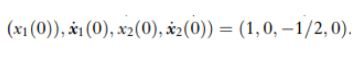
\includegraphics[height=2cm]{ec15.png}
\end{center}

El codigo sigueinte es muy similar al utilizado en la actividad 6 con ecepcion que se agregaron los parametros $u1$ y $u2$

\begin{center}
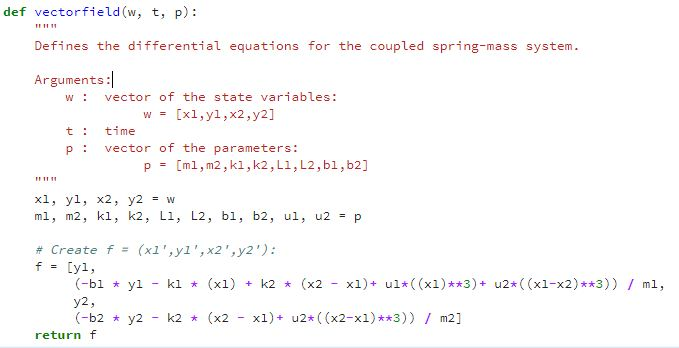
\includegraphics[height=8cm]{cod7.png}
\end{center}


\begin{center}
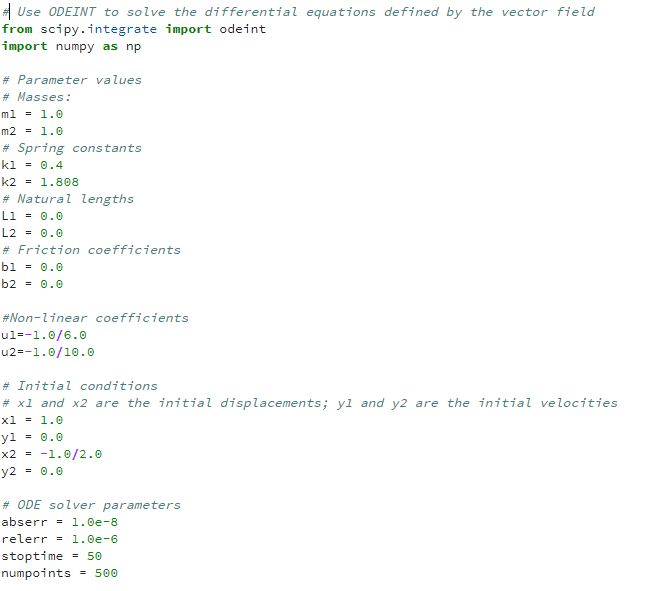
\includegraphics[height=12cm]{cod8.png}
\end{center}
\begin{center}
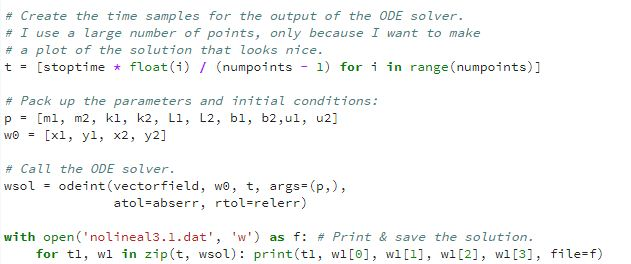
\includegraphics[height=7cm]{cod9.png}
\end{center}

Las graficas que se llevaron a cabo en este problema son las siguientes:

\begin{center}
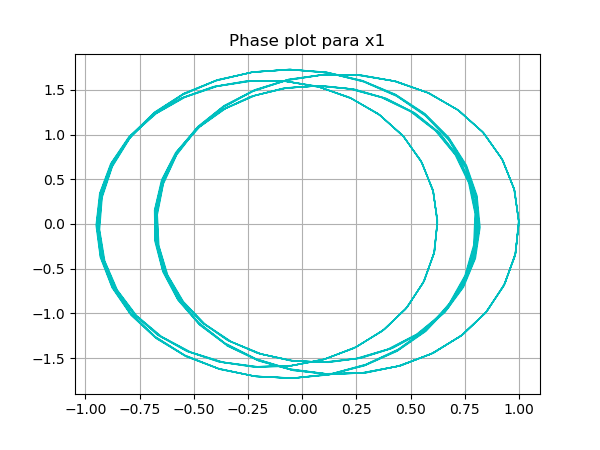
\includegraphics[height=7cm]{nolineal3_1_1.png}
\end{center}

\begin{center}
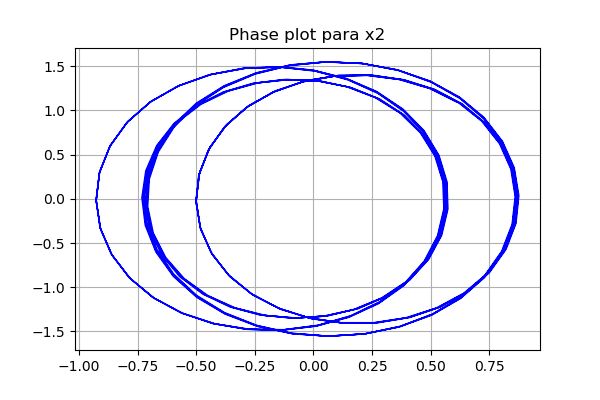
\includegraphics[height=7cm]{nolineal3_1_2.png}
\end{center}

\begin{center}
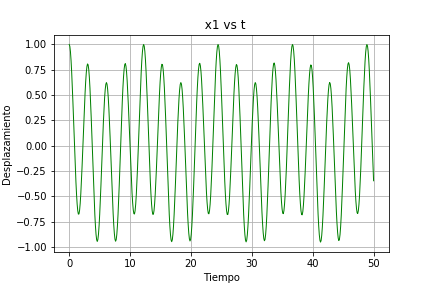
\includegraphics[height=7cm]{nolineal3_1_3.png}
\end{center}

\begin{center}
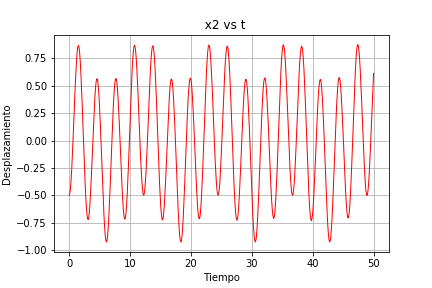
\includegraphics[height=7cm]{nolineal3_1_4.png}
\end{center}

\begin{center}
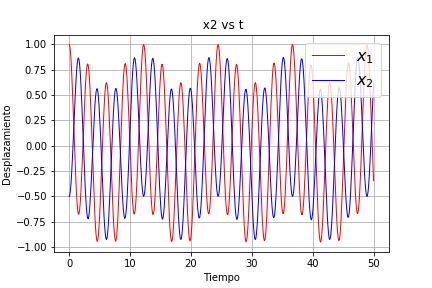
\includegraphics[height=7cm]{nolineal3_1_5.png}
\end{center}

\begin{center}
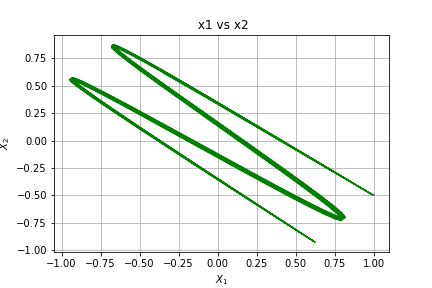
\includegraphics[height=7cm]{nolineal3_1_6.png}
\end{center}

%%%%%%%%%%%%%%%%%%%%%%%%%%%%%%%%%%%%%%%%%%%%%%
\subsection{Ejemplo 3.2}

Suponga que $m1=m2=1$. Describa el movimiento de las constantes de resorte $k1=0.4$ y $k2=1.808$, coeficientes de amortiguación b1=0 y b2=0, coefecientes no lineales $u1=-1/6$ y $u2=-1/10$ , con condiciones iniciales:



\begin{center}
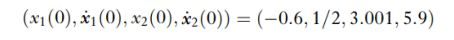
\includegraphics[height=1cm]{ec16.png}
\end{center}

En este ejemplo el segmento del codigo es el mismo solamente cambiando las condiciones iniciales que ofrece el problema

Las graficas que se llevaron a cabo en este problema son las siguientes:


\begin{center}
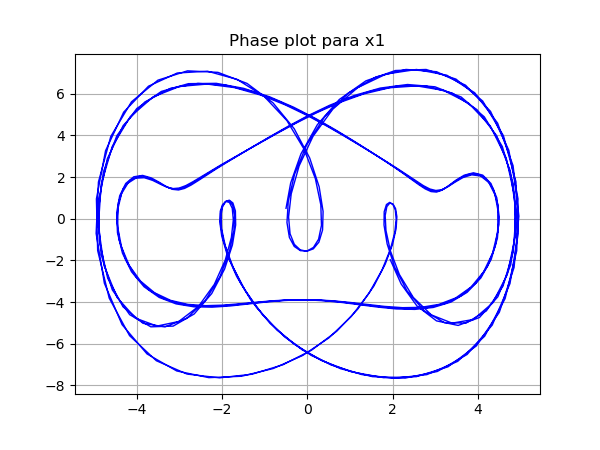
\includegraphics[height=7cm]{nolineal3_2_1.png}
\end{center}

\begin{center}
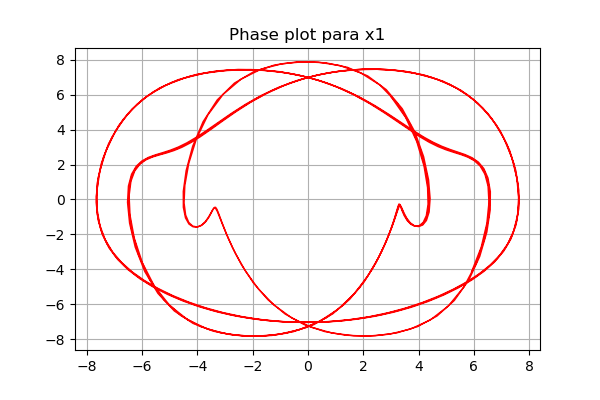
\includegraphics[height=7cm]{nolineal3_2_2.png}
\end{center}

\begin{center}
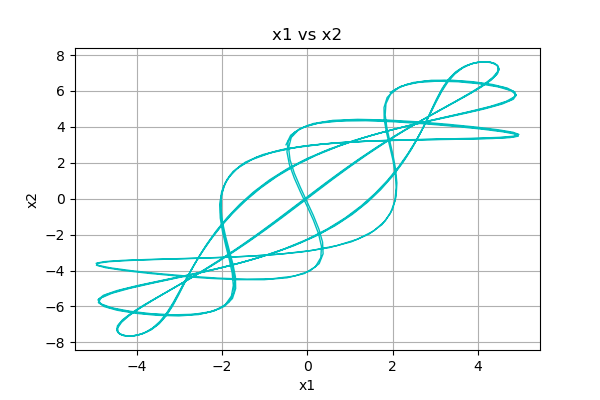
\includegraphics[height=7cm]{nolineal3_2_3.png}
\end{center}

%%%%%%%%%%%%%%%%%%%%%%%%%%%%%%%%%%%%%%%%%%%%%%
\subsection{Ejemplo 3.3}

Suponga que $m1=m2=1$. Describa el movimiento de las constantes de resorte $k1=0.4$ y $k2=1.808$, coeficientes de amortiguación b1=0 y b2=0, coefecientes no lineales $u1=-1/6$ y $u2=-1/10$ , con condiciones iniciales, para este ejemplo de igual manera no se presenta el segmento del codigo debido aque es el mismo simplemente cambiando las condiciones iniciales.


Las graficas que se realizaron en este ejemplo son las siguientes:

\begin{center}
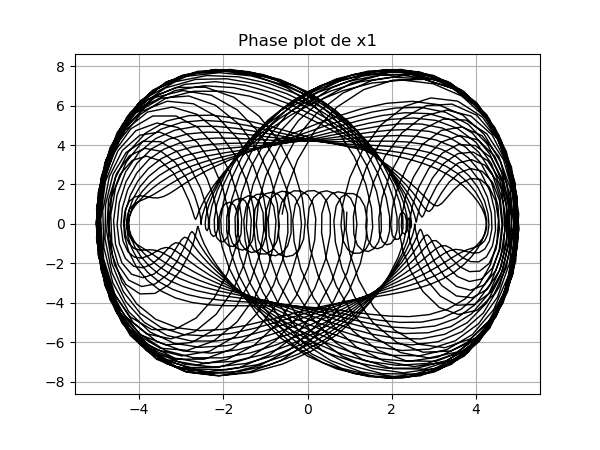
\includegraphics[height=7cm]{nolineal3_3_1.png}
\end{center}

\begin{center}
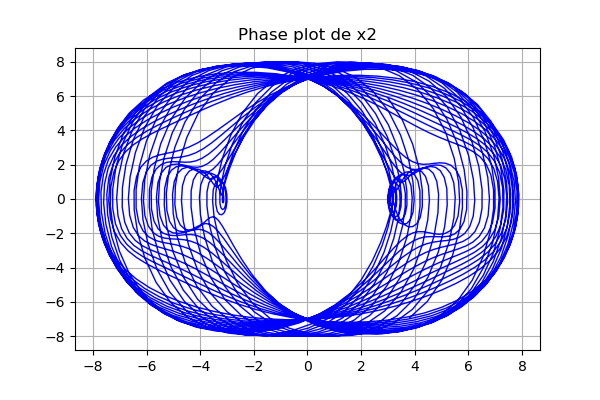
\includegraphics[height=7cm]{nolineal3_3_2.png}
\end{center}

\begin{center}
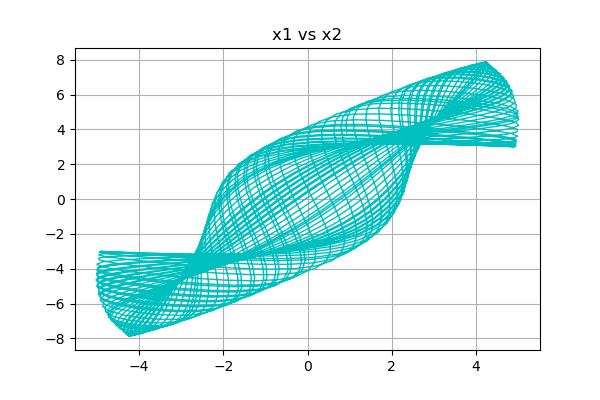
\includegraphics[height=7cm]{nolineal3_3_3.png}
\end{center}

%%%%%%%%%%%%%%%%%%%%%%%%%%%%%%%%%%%%%%%%%%%%%%%%%%%
\section{Añadiendo forzamiento}

En esta parte del texto habla de un sistema o modelo de forzamiento externo y da un ejemplo como el sinusoidal que tiene la forma $Fcoswt$ y se obtendra las siguintes ecuaciones diferenciales:

\begin{center}
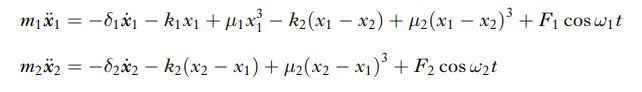
\includegraphics[height=2cm]{ec17.png}
\end{center}

En el codigo se agregaran los parametros f1,f2 y w1,w2
como a continuacion se muestra en la imagen:


\begin{center}
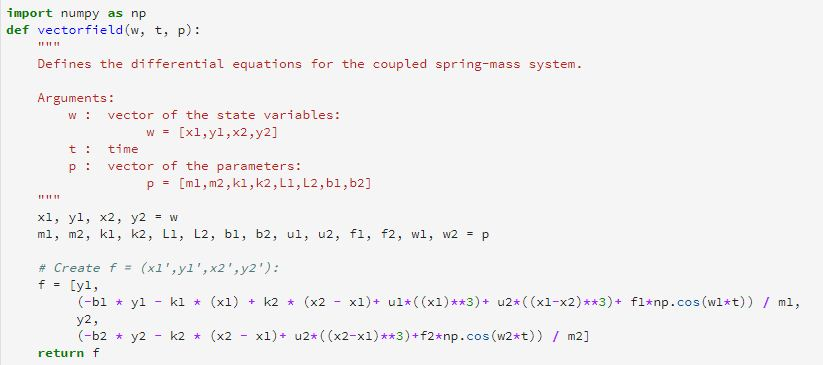
\includegraphics[height=8cm]{cod10.png}
\end{center}

\begin{center}
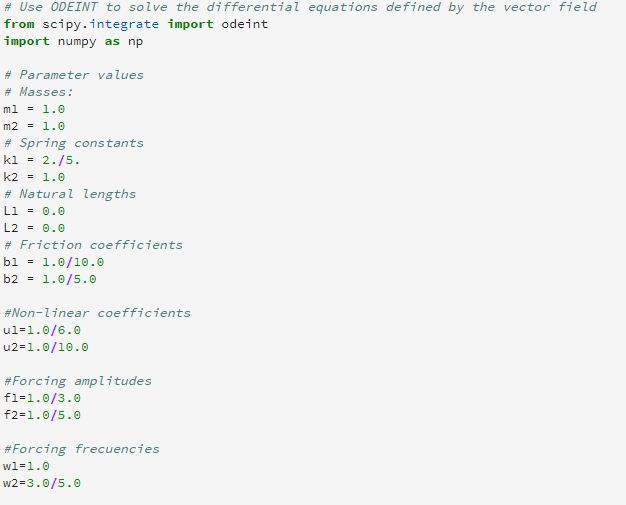
\includegraphics[height=8cm]{cod11.png}
\end{center}


Acontinuacion se mostraran las graficas que se realizaron en este ejemplo:

\begin{center}
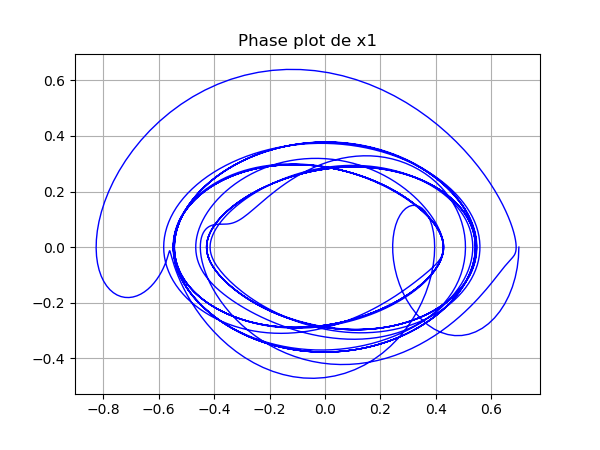
\includegraphics[height=7cm]{nolineal4_1_1.png}
\end{center}

\begin{center}
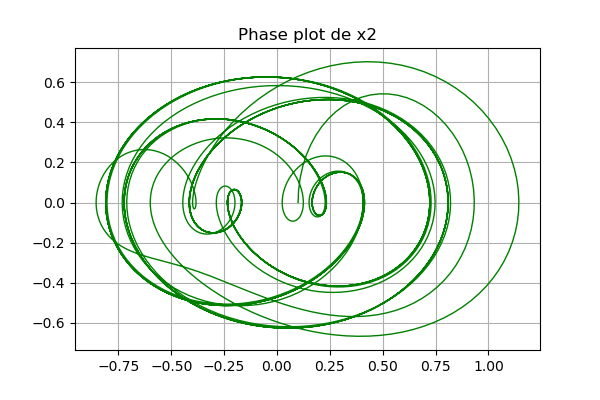
\includegraphics[height=7cm]{nolineal4_1_2.png}
\end{center}


\begin{center}
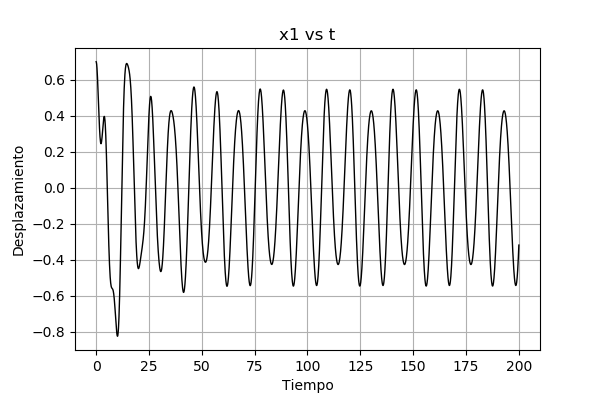
\includegraphics[height=7cm]{nolineal4_1_3.png}
\end{center}

\begin{center}
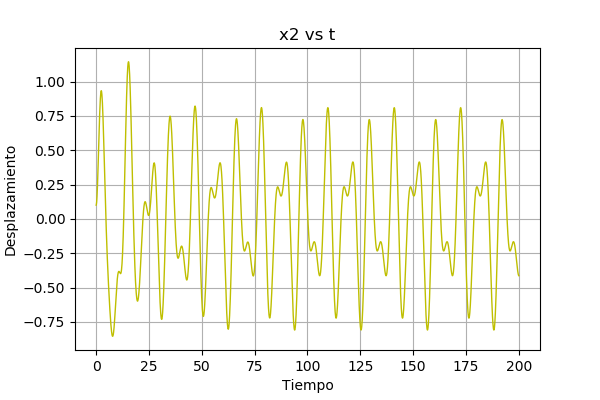
\includegraphics[height=7cm]{nolineal4_1_4.png}
\end{center}

\begin{center}
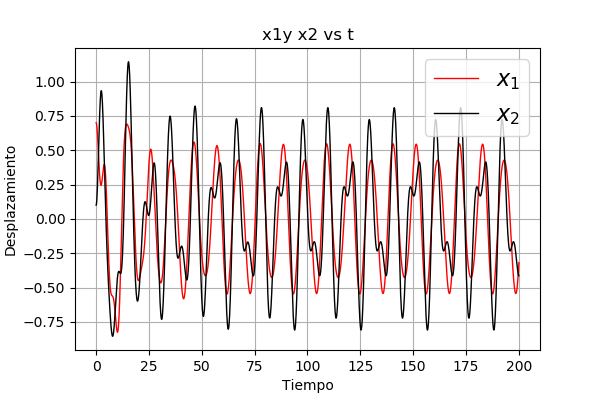
\includegraphics[height=7cm]{nolineal4_1_5.png}
\end{center}

\begin{center}
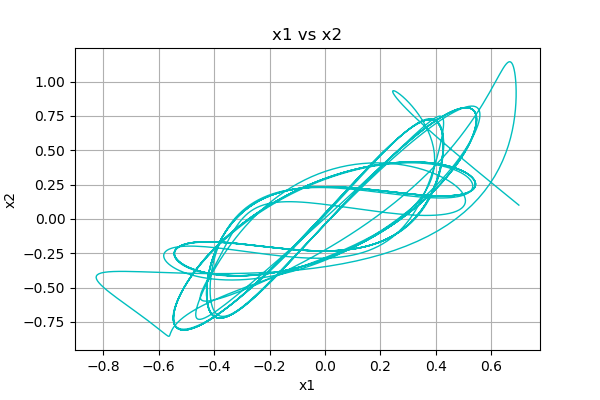
\includegraphics[height=7cm]{nolineal4_1_6.png}
\end{center}


\section{Conclusión}

Me paracio muy interesante esta actividad ya que fue un poco diferente a lo de la actividad 6, un poco mas complejo, y la graficas mas "feas"

\section{Bibliografia}

couple spring equations,TEMPLE H. FAY and SARAH DUNCAN GRAHAM,publicado 12 de septiembre del 2012
$http://math.oregonstate.edu/~gibsonn/Teaching/MTH323-010S15/Supplements/coupled_spring.pdf$














\end{document}
